%
% Copyright 2018 Joel Feldman, Andrew Rechnitzer and Elyse Yeager.
% This work is licensed under a Creative Commons Attribution-NonCommercial-ShareAlike 4.0 International License.
% https://creativecommons.org/licenses/by-nc-sa/4.0/
%
\questionheader{ex:s2.2}

Recall that we are using $\log x$ to denote the logarithm of $x$ with
base $e$. In other courses it is often denoted $\ln x$.

%%%%%%%%%%%%%%%%%%
\subsection*{\Conceptual}
%%%%%%%%%%%%%%%%%%


\begin{Mquestion}\label{prob_s2.2:avgvalue}
Below is the graph of a function $y=f(x)$. Its average value on the interval  $[0,5]$ is $A$. Draw a rectangle on the graph with area $\int_0^5 f(x)\,\dee{x}$.
\begin{center}
\begin{tikzpicture}
\YEaaxis{1}{7}{2}{3}
\draw[thick, blue] plot[domain=0:6.28, samples=100](\x,{-.5*\x*sin(\x r)});
\YExcoord{6.28}{5}
\YEycoord{1}{A}
\end{tikzpicture}
\end{center}
\end{Mquestion}
\begin{hint}
See Definition~\eref{CLP101}{def:AVaverage} in the CLP--II text and the discussion following it for the link between area under the curve and averages.
\end{hint}
\begin{answer}
The most straightforward of many possible answers is shown.
\begin{center}
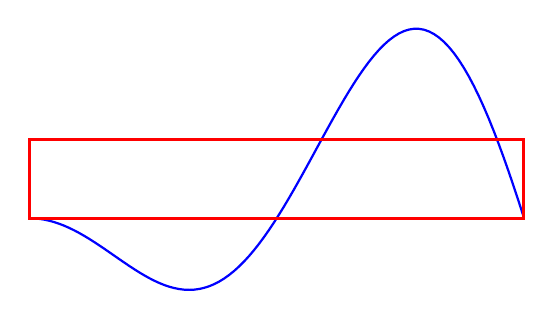
\begin{tikzpicture}
\YEaaxis{1}{7}{2}{3}
\draw[thick, blue] plot[domain=0:6.28, samples=100](\x,{-.5*\x*sin(\x r)});
\YExcoord{6.28}{5}
\YEycoord{1}{A}
\draw[very thick, red] (0,0) rectangle (6.28,1);
\end{tikzpicture}
\end{center}
\end{answer}
\begin{solution}
Since the average of $f(x)$ on the interval $[0,5]$ is $A$, using Definition~\eref{CLP101}{def:AVaverage} in the CLP--II text,
\begin{align*}
A&=\frac{1}{5}\int_0^5 f(x)\,\dee{x}\\
5A&=\int_0^5 f(x)\,\dee{x}
\end{align*}
So, a rectangle with width 5 and height $A$ has area
$\int_0^5 f(x)\,\dee{x}$.

That is: if we replace $f(x)$ with the constant function $g(x)=A$, then on the interval $[0,5]$, the area under the curve is unchanged.

\begin{center}
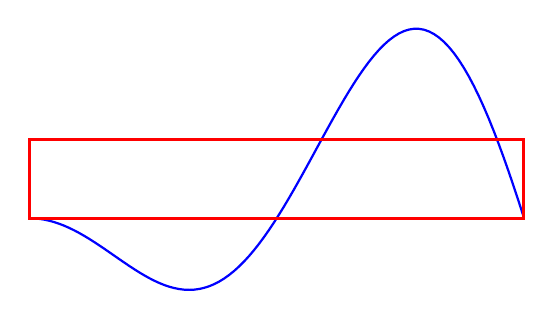
\begin{tikzpicture}
\YEaaxis{1}{7}{2}{3}
\draw[thick, blue] plot[domain=0:6.28, samples=100](\x,{-.5*\x*sin(\x r)});
\YExcoord{6.28}{5}
\YEycoord{1}{A}
\draw[very thick, red] (0,0) rectangle (6.28,1);
\end{tikzpicture}
\end{center}

(There are many rectangles with area $5A$; we drew the one we consider to be the most straightforward in this context.)
\end{solution}
%%%%%%%%%%%%%%%%%%%
\begin{question}\label{prob_s2.2:vel}
Suppose a car travels for 5 hours in a straight line, with an average velocity of 100 kph. How far did the car travel?
\end{question}
\begin{hint}
Average velocity is discussed in Example~\eref{CLP101}{eg:AVvelocity} of the CLP--II text.
You don't need an integral for this.
\end{hint}
\begin{answer}
500 km
\end{answer}
\begin{solution}
Average velocity,  as discussed in Example~\eref{CLP101}{eg:AVvelocity} of the CLP--II text,
is change in position divided by change in time. So, the change in position (i.e. distance travelled) is (100 km/h)(5 h) = 500 km.
\end{solution}
%%%%%%%%%%%%%%%%%%%


\begin{question}
A force $F(x)$ acts on an object from position $x=a$ metres to position $x=b$ metres, for a total of $W$ joules of work. What was the average force on the object?
\end{question}
\begin{hint}
Much like Problem~\ref{prob_s2.2:vel}, you don't need to do any integration here.
\end{hint}
\begin{answer}
$\dfrac{W}{b-a}$ N
\end{answer}
\begin{solution}
The work done is
\[W=\int_a^b F(x)\,\dee{x}\]
so the average value of $F(x)$ is
\[\frac{1}{b-a}\int_a^b F(x)\,\dee{x} =\frac{1}{b-a}(W).\]
We can quickly check our units: since $W$ is in joules  (that is, newton-metres), and $b-a$ is in metres, so $\frac{W}{b-a}$ is in newtons.

\end{solution}
%%%%%%%%%%%%%%%%%%%

\begin{question}
Suppose we want to approximate the average value of the function $f(x)$ on the interval $[a,b]$. To do this, we cut the interval $[a,b]$ into $n$ pieces, then take $n$ samples by finding the function's output at the left endpoint of each piece, starting with $a$. Then, we average those $n$ samples. (In the example below, $n=4$.)
\begin{center}
\begin{tikzpicture}
\YEaaxis{1}{6.5}{1}{3}
\draw[thick, blue] plot[domain=-1:6.25, samples=100](\x,{sin(\x r)+\x*\x/15});
\YExcoord{1}{a}
\YExcoord{5}{b}
\color{red}
\draw (3,3) node[shape=rectangle, above](A){average these $y$-values};
\foreach \x/\y in {1/0.91,2/1.18,3/0.74,4/0.31}
	{\draw (\x,\y) node[vertex](v\x){};
	\draw (v\x)+(0,.25) node(w\x){};
	\draw[->, thick] (A) -- (w\x);}
\end{tikzpicture}
\end{center}
\begin{enumerate}[(a)]
\item Using $n$ samples, what is the distance between two consecutive sample points $x_i$ and $x_{i+1}$?
\item Assuming $n \geq 4$, what is the $x$-coordinate of the fourth sample?
\item Assuming $n \geq 4$, what is the $y$-value of the fourth sample?
\item Write the approximation of the average value of $f(x)$ over the interval $[a,b]$ using sigma notation.
\end{enumerate}
\end{question}
\begin{hint}
Part (a) is asking the length of the pieces we've cut our interval into. Part (c) should be given in terms of $f$.
 Our final answer in (d) will resemble a Riemann sum, but without some extra manipulation it won't be in exactly the form of a Riemann sum we're used to.
\end{hint}
\begin{answer}
(a) $\dfrac{b-a}{n}$\qquad (b) $a+3\dfrac{b-a}{n} $ \qquad
(c) $f\left(a+3\dfrac{b-a}{n} \right)$ \qquad (d)
$\dfrac{1}{n}\sum\limits_{i=1}^n f\left(a+(i-1)\frac{b-a}{n}\right)$
\end{answer}
\begin{solution}
\begin{enumerate}[(a)]
\item The entire interval has length $b-a$, and we're cutting it into $n$ pieces, so the length of one piece (and hence the distance between two consecutive samples) is $\frac{b-a}{n}$.
\item The first sample, as given in the question statement, is taken at $x=a$. The second sample, then, is at $x=a+\frac{b-a}{n}$, this third is at $x=1+2\frac{b-a}{n}$, and the fourth is at $a+3\frac{b-a}{n}$.
\item The $y$-value of the fourth sample is simply $f\left(a+3\frac{b-a}{n}\right)$. Note this is the number we use in our average, not the $x$-value.
\item Our samples are $f(a)$, $f\left(a+\frac{b-a}{n}\right)$,
$f\left(a+2\frac{b-a}{n}\right)$,
$f\left(a+3\frac{b-a}{n}\right)$, etc. Since there are $n$ of them, we divide their sum by $n$. So, the average is:
\begin{align*}
&~\frac{f(a)+f\left(a+\frac{b-a}{n}\right)+
f\left(a+2\frac{b-a}{n}\right)+\cdots + f\left(a+(n-1)\frac{b-a}{n}\right)}{n}\\
&=\frac{1}{n}\left[f(a)+f\left(a+\frac{b-a}{n}\right)f\left(a+2\frac{b-a}{n}\right)+\cdots + f\left(a+(n-1)\frac{b-a}{n}\right)\right]\\
&= \frac{1}{n}\sum_{i=1}^nf\left(a+(i-1)\frac{b-a}{n}\right)
\intertext{Remark: if we multiply and divide by $b-a$, we see this expression is equivalent to a left Riemann sum, divided by the length of our interval.}
&= \frac{1}{b-a}\sum_{i=1}^nf\left(a+(i-1)\frac{b-a}{n}\right)\frac{b-a}{n}\\
&= \frac{1}{b-a}\sum_{i=1}^nf\left(a+(i-1)\De x\right)\De x
\end{align*}
As $n$ gets larger and larger, using the definition of a definite integral, this expression gets closer and closer to $\frac{1}{b-a}\int_a^bf(x)\,\dee{x}$. This is one way of justifying our definition of an average of a function on an interval.
\end{enumerate}
\end{solution}

%%%%%%%%%%%%%%%%%%%
\begin{Mquestion}
Suppose $f(x)$ and $g(x)$ are functions that are defined for all numbers in the interval $[0,10]$.
\begin{enumerate}[(a)]
\item  If $f(x) \leq g(x)$ for all $x$ in $[0,10]$, then is the average value of $f(x)$ is less than or equal to the average value of $g(x)$ on the interval $[0,10]$, or is there not enough information to tell?
\item Suppose $f(x) \leq g(x)$ for all $x$ in $[0.01,10]$. Is the average value of $f(x)$ less than or equal to the average value of $g(x)$ over the interval $[0,10]$, or is there not enough information to tell?
\end{enumerate}
\end{Mquestion}
\begin{hint}
For (b), the value of $f(0)$ could be much, much larger than $g(0)$.
\end{hint}
\begin{answer}
(a) yes \qquad (b) not enough information
\end{answer}
\begin{solution}
\begin{enumerate}[(a)]
\item Yes, the average of $f(x)$ is less than or equal to the average of $g(x)$ on $[0,10]$. The reason is that, if $f(x) \leq g(x)$ for all $x$ in $[0,10]$, then:
\[\frac{1}{10}\int_0^{10}f(x)\,\dee{x} \leq \frac{1}{10}\int_0^{10}g(x)\,\dee{x}.\]
\item There is not enough information to tell. It's certainly possible: for instance, take $f(x)=0$ and $g(x)=1$ for all $x$ in $[0,10]$. Then $f(x) \leq g(x)$ and the average of $f(x)$ is 0, which is less than 1, the average of $g(x)$.

However, consider $f(x) = \begin{cases}
100 & \text{ if } 0 \le x \le 0.01\\
0 & \text{ else }
\end{cases}$ and $g(x) = 0$. Then $f(x) \le g(x)$ for all $x$ in $[0.01,10]$, but the average of $f(x)$ is $0.1$, while the average of $g(x)$ is 0.
\end{enumerate}
\end{solution}
%%%%%%%%%%%%%%%%%%%

\begin{question}
Suppose $f$ is an odd function, defined for all real numbers. What is the average of $f$ on the interval $[-10,10]$?
\end{question}
\begin{hint}
The answer is something very simple.
\end{hint}
\begin{answer}
0
\end{answer}
\begin{solution}
Recall the definition of an odd function: $f(-x)=-f(x)$. Since the domain of integration is symmetric, the signed area on one side of the $y$-axis ``cancels out" the signed area on the other--this is Theorem~\eref{CLP101}{thm:INTevenodd} in the CLP--II text.
\begin{align*}\frac{1}{20}\int_{-10}^{10}f(x)\,\dee{x}&=\frac{1}{20}(0)=0
\end{align*}
\end{solution}
%%%%%%%%%%%%%%%%%%%



%%%%%%%%%%%%%%%%%%
\subsection*{\Procedural}
%%%%%%%%%%%%%%%%%%

\begin{Mquestion}[2016Q3]
Find the average value of $f(x) = \sin(5x)+1$ over the interval $-\pi/2 \le x \le \pi/2 $.
\end{Mquestion}

\begin{hint}
Apply the definition of ``average value'' in Section~\eref{CLP101}{sec avg} of the
%\href{http://www.math.ubc.ca/%7Efeldman/m101/clp/clp_notes_101.pdf}{CLP--II text}.
CLP--II text.
\end{hint}

\begin{answer}
$1$
\end{answer}

\begin{solution}
By definition, the average value is
\begin{align*}
 \frac{1}{\pi}\int_{-\pi/2}^{\pi/2} \big( \sin(5x)+1 \big) \,\dee{x}
\end{align*}
We now observe that $\sin(5x)$ is an odd function, and hence its integral over the symmetric interval $[-\frac\pi2,\frac\pi2]$ equals zero. So the average value of $f(x)$ on this interval is $1$:
\begin{align*}
 \frac{1}{\pi}\int_{-\pi/2}^{\pi/2} \big( \sin(5x)+1 \big) \,\dee{x}&=
  \frac{1}{\pi}\int_{-\pi/2}^{\pi/2}  \sin(5x) \,\dee{x}+ \frac{1}{\pi}\int_{-\pi/2}^{\pi/2}1 \,\dee{x}\\
  &= \frac{1}{\pi}\int_{-\pi/2}^{\pi/2}1 \,\dee{x}=1
\end{align*}
Alternatively, using the fundamental theorem of calculus, the average equals:
\begin{align*}
\frac{1}{\pi}\bigg[\frac{-\cos (5x) }{5} +x  \bigg]_{-\pi/2}^{\pi/2}
= \frac{1}{\pi}\bigg\{\bigg[\frac{-\cos (5\pi/2) }{5} +\frac{\pi}{2}\bigg]
   -\bigg[ \frac{-\cos (-5\pi/2) }{5} + \frac{-\pi}{2} \bigg]\bigg\}
= \frac{\pi }{\pi}=1
\end{align*}

\end{solution}
%%%%%%%%%%%%%%%%%%%


\begin{question}[2015A]
Find the average value of the function $y= x^2\log x$ on the interval
$1 \le x\le e$.
\end{question}

\begin{hint}
You can antidifferentiate $x^2\log x$ using integration by parts.
\end{hint}

\begin{answer}
$\displaystyle\frac{1}{e-1}\Big[\frac{2}{9}e^3+\frac{1}{9}\Big]$
\end{answer}

\begin{solution}
By definition, the average is
\begin{align*}
\frac{1}{e-1}\int_1^e x^2\log x\ \dee{x}
  &
  \intertext{To antidifferentiate, we use integration by parts with $u=\log x$ and $\dee{v}=x^2\,\dee{x}$, hence $\dee{u}=\frac{1}{x}\,\dee{x}$ and $v=\frac{1}{3}x^3$.}
  \frac{1}{e-1}\int_1^e x^2\log x\ \dee{x}&=
\frac{1}{e-1}\left(\left[\frac{1}{3}x^3\log x\right]_1^e - \int_1^e \frac{1}{3}x^2\,\dee{x}  \right)
  \\&=
  \frac{1}{e-1}\bigg[\frac{x^3}{3}\log x-\frac{x^3}{9}\bigg]_{x=1}^{x=e}\\
  &=\frac{1}{e-1}\bigg[\frac{e^3}{3}-\frac{e^3}{9}+\frac{1}{9}\bigg]\\
  &=\frac{1}{e-1}\bigg[\frac{2}{9}e^3+\frac{1}{9}\bigg]
\end{align*}

\end{solution}
%%%%%%%%%%%%%%%%%%%

\begin{question}[2016A]
Find the average value of the function $f(x) = 3\cos^3x + 2\cos^2x$ on the interval $0\le x\le\frac\pi2$.
\end{question}

\begin{hint}
You can antidifferentiate an odd power of cosine with a substitution; for an even power of cosine, use the identity $\cos^2 x = \frac{1}{2}\big(1+\cos(2x)\big)$.
\end{hint}

\begin{answer}
$\dfrac{4}{\pi}+1$
\end{answer}

\begin{solution}
By definition, the average value in question equals
\begin{equation*}
\frac1{\pi/2-0} \int_0^{\pi/2} ( 3\cos^3x + 2\cos^2x ) \,\dee{x}
= \frac2\pi \bigg( \int_0^{\pi/2} 3\cos^3x \,\dee{x} + \int_0^{\pi/2} 2\cos^2x \,\dee{x} \bigg)
\end{equation*}
For the first integral we use the substitution $u = \sin x$,
$\dee{u}=\cos x\,\dee{x}$, $\cos^2 x=1-\sin^2 x = 1-u^2$.
Note that the endpoints
$x=0$ and $x=\frac\pi2$ become $u=0$ and $u=1$, respectively.
\begin{align*}
\int_0^{\pi/2} 3 \cos^3x \,\dee{x}
&= \int_0^{\pi/2} 3 \cos^2 x \cos x \,\dee{x} \\
&= \int_0^{1} 3(1-u^2) \,\dee{u} \\
&= (3u-u^3)\Big|_0^1 = 2.
\end{align*}
For the second integral we use the trigonometric identity
$\cos^2x\,\dee{x} = \frac{1 + \cos(2x)}{2}$.
\begin{align*}
2 \int_0^{\pi/2} \cos^2x\,\dee{x}
&= \int_0^{\pi/2} \big(1 + \cos(2x) \big) \,\dee{x} \\
&= \bigg[ x + \frac{1}{2}\sin(2x) \bigg]_0^{\pi/2}
= \frac\pi2
\end{align*}
Therefore, the average value in question is
\begin{equation*}
\frac2\pi \bigg( \int_0^{\pi/2} 3\cos^3x \,\dee{x} + \int_0^{\pi/2} 2\cos^2x \,\dee{x} \bigg)
= \frac2\pi \bigg( 2 + \frac\pi2 \bigg)
= \frac{4}{\pi}+1.
\end{equation*}


\end{solution}
%%%%%%%%%%%%%%%%%%%


\begin{question}[2012A]
Let $k$ be a positive constant.
Find the average value of the function $f(x) = \sin(kx)$ on the interval
$0\le x\le \pi/k$.
\end{question}

\begin{hint}
If you're not sure how to antidifferentiate, try the substitution $u=kx$, $\dee{u}=k\dee{x}$, keeping in mind that $k$ is a constant. Interestingly, your final answer won't depend on $k$.
\end{hint}

\begin{answer}
 $\dfrac{2}{\pi}$
\end{answer}

\begin{solution}
By definition, the average value in question equals
\begin{equation*}
\text{Ave}=\frac1{\pi/k-0} \int_0^{\pi/k} \sin(kx) \,\dee{x}
\end{equation*}
To evaluate the integral, we use the substitution $u = kx$,
$\dee{u}=k\,\dee{x}$.
Note that the endpoints
$x=0$ and $x=\pi/k$ become $u=0$ and $u=\pi$, respectively. So
\begin{align*}
\text{Ave}=\frac{k}{\pi} \int_0^\pi \sin(u) \,\frac{\dee{u}}{k}
=\frac{1}{\pi}\Big[-\cos(u)\Big]_0^\pi
=\frac{2}{\pi}
\end{align*}

Remark: the average does not depend on $k$. To see why this is, note that $\sin(kx)$ runs between $-1$ and $1$ as $x$ changes. When $x=0$, $kx=0$, and when $x=\pi/k$, $kx=\pi$. So, our function $\sin (kx)$ runs exactly from $\sin  0 =0$ to $\sin(\pi/2)=1$, then back down to $\sin\pi=0$.

\begin{center}
\begin{tikzpicture}
\YEaaxis{1}{7}{1}{2.5}
\YExcoord{6.28}{\frac{\pi}{k}}
\YExcoord{3.14}{\frac{\pi}{2k}}
\YEycoord{2}{1}
\draw[thick, blue] plot[domain=0:3.14]({2*\x},{2*sin(\x r)}) node[above right]{$y=\sin(k x)$};
\end{tikzpicture}
\end{center}
\end{solution}
%%%%%%%%%%%%%%%%%%%



\begin{Mquestion}[1997A]
 The temperature in Celsius in a 3 m long rod at a point $x$ metres from the left end of the rod is given by the
function $T(x)=\frac{80}{16-x^2}$. Determine the average temperature in the rod.
\end{Mquestion}

\begin{hint}
The method of partial fractions can help you antidifferentiate.
\end{hint}

\begin{answer}
$\dfrac{10}{3}\log 7$ degrees Celsius
\end{answer}

\begin{solution}
By definition, the average temperature is
\[\frac{1}{3}\int_0^3 T(x)\,\dee{x}
=\frac{1}{3}\int_0^3 \frac{80}{16-x^2}\,\dee{x}\]
We don't see an obvious substitution, but  integrand is a rational function. The degree of the numerator is strictly less than the degree of the denominator, so we factor the denominator and use a partial fraction decomposition.

\begin{align*}
\frac{80}{16-x^2}&=\frac{80}{(4-x)(4+x)} = \frac{A}{4-x}+\frac{B}{4+x}\\
80&=A(4+x)+B(4-x)
\intertext{
Setting $x=4$, we see $80=8A$, so \textcolor{red}{$A=10$}. Setting $x=-4$, we see $80=8B$, so \textcolor{red}{$B=10$}.
}
\frac{1}{3}\int_0^3 \frac{80}{16-x^2}\,\dee{x}&=\frac{1}{3}\int_0^3 \frac{80}{(4-x)(4+x)}\,\dee{x}=\frac{1}{3}\int_0^3 \Big[\frac{\textcolor{red}{10}}{4-x}+\frac{\textcolor{red}{10}}{4+x}\Big]\,\dee{x}\\
&=\frac{1}{3}\int_0^3 \Big[-\frac{10}{x-4}+\frac{10}{4+x}\Big]\,\dee{x}\\
&=\frac{10}{3}\Big[-\log|x-4|+\log|x+4|\Big]_0^3 \\
&=\frac{10}{3}\log\Big|\frac{x+4}{x-4}\Big|\bigg|_0^3
=\frac{10}{3}[\log 7-\log 1] \\
&=\frac{10}{3}\log 7\quad\text{ degrees Celsius}
\end{align*}
\end{solution}
%%%%%%%%%%%%%%%%%%%

\begin{question}[1997D]
What is the average value of the function
$f(x)=\dfrac{\log x}{x}$ on the interval $[1,e]$?
\end{question}

\begin{hint}
Try the substitution $u=\log x$, $\dee{u}=\frac{1}{x}\,\dee{x}$.
\end{hint}

\begin{answer}
$\dfrac{1}{2(e-1)}$
\end{answer}

\begin{solution}
By definition, the average value is
\begin{align*}
\frac{1}{e-1}\int_1^e\frac{\log x}{x}\ \dee{x}&
\intertext{To integrate, we use the substitution $u=\log x$, $\dee{u}=\frac{1}{x}\,\dee{x}$.
Then the limits of integration become 0 and 1, respectively.}
\frac{1}{e-1}\int_1^e\frac{\log x}{x}\ \dee{x}&
=\frac{1}{e-1}\int_0^1u\ \dee{u}
=\frac{1}{e-1}\bigg[\frac{u^2}{2}\bigg]_0^1
=\frac{1}{2(e-1)}
\end{align*}
\end{solution}
%%%%%%%%%%%%%%%%%%%


\begin{question}[2000D]
 Find the average value of $f(x)=\cos^2(x)$ over $0\le x\le 2\pi$.
\end{question}

\begin{hint}
Remember $\cos^2 x = \frac{1}{2}\big(1+\cos(2x)\big)$.
\end{hint}

\begin{answer}
$\dfrac12$
\end{answer}

\begin{solution}
By definition, the average value is:
\begin{align*}
\frac{1}{2\pi}\int_0^{2\pi}\cos^2x\,\dee{x}
=\frac{1}{2\pi}\cdot\frac{1}{2}\int_0^{2\pi}\big(\cos(2x)+1\big)\,\dee{x}
=\frac{1}{4\pi}\Big[\frac{\sin(2x)}{2}+x\Big]_0^{2\pi}
=\frac{1}{4\pi}\cdot 2\pi
=\frac{1}{2}
\end{align*}

\end{solution}
%%%%%%%%%%%%%%%%%%%





\begin{Mquestion}
The carbon dioxide concentration in the air at a particular location over one year is approximated by $C(t) = 400+50\cos\left(\frac{t}{12}\pi\right)+200\cos\left(\frac{t}{4380}\pi\right)$ parts per million, where  $t$ is measured in hours.
\begin{enumerate}[(a)]
\item  What is the average carbon dioxide concentration for that location for that year?
\item What is the average over the first day? \item Suppose measurements were only made at noon every day: that is, when $t=12+24n$, where $n$ is any whole number between 0 and 364.
Then the daily variation would cease: $50\cos\left(\frac{(12+24n)}{12}\pi\right) = 50\cos\left(\pi+2\pi n\right) = 50\cos\pi=-50$. So, the approximation for the concentration of carbon dioxide in the atmosphere might be given as
\[N(t) = 350 +200\cos\left(\frac{t}{4380}\pi\right)\quad\text{ ppm}\]
What is the relative error in the yearly average concentration of carbon dioxide involved in using $N(t)$, instead of $C(t)$?
\end{enumerate}
You may assume a day has exactly 24 hours, and a year has exactly 8760 hours.
\end{Mquestion}
\begin{hint}
Notice the term $50\cos\left(\frac{t}{12}\pi\right)$ has a period of 24 hours, while the term
$200\cos\left(\frac{t}{4380}\pi\right)$ has a period of one year.

If $n$ is an approximation of $c$, then the relative error of $n$ is $\frac{|n-c|}{c}$.
\end{hint}
\begin{answer}
(a) 400 ppm \qquad (b) $\approx 599.99$ ppm
\qquad (c) 0.125, or 12.5\%
\end{answer}
\begin{solution}
Before we start answering questions, let's look at our function a little more carefully.
The term $50\cos\left(\frac{t}{12}\pi\right)$ has a period of 24 hours, while the term
$200\cos\left(\frac{t}{4380}\pi\right)$ has a period of one year. So, the former term describes a standard daily variation, while the latter gives a seasonal variation over the year.

(a) Using the definition of an average, the average concentration over one year ($t=0$ to $8760$) is:
\begin{align*}
&\frac{1}{8760}\int_0^{8760}\left(400+\textcolor{red}{50\cos\left(\frac{t}{12}\pi\right)}+\textcolor{blue}{200\cos\left(\frac{t}{4380}\pi\right)}\right)\,\dee{t}\\
&=\frac{1}{8760}\int_0^{8760}400\,\dee{t}
+
\textcolor{red}{\frac{50}{8760}\int_0^{8760}\cos\left(\frac{t}{12}\pi\right)\,\dee{t}}
+
\textcolor{blue}{\frac{200}{8760}\int_0^{8760}\cos\left(\frac{t}{4380}\pi\right)\,\dee{t}}\\
&= 400 +\textcolor{red}{ \frac{5}{876}\left[\frac{12}{\pi}\sin\left(\frac{t}{12}\pi\right)\right]_0^{8760}}+
\textcolor{blue}{\frac{5}{219}\left[\frac{4380}{\pi}\sin\left(\frac{t}{4380}\pi\right)\right]_0^{8760}}
\intertext{Since $\frac{8760}{12} = 730$, which is even, $\sin\left(\frac{8760}{12}\pi\right)=\sin(0)=0$. Also, $\sin\left(\frac{8760}{4380}\pi\right)=\sin(2\pi)=0$. }
&=400+\textcolor{red}{\frac{5}{876}(0}) + \textcolor{blue}{\frac{5}{219}(0)}\\
&=400\quad\text{ ppm}
\end{align*}
Remark: for the portions of the integral in red and blue, we also could have noticed that the integrand goes through a whole (integer) number of periods. For every period, the net signed area between the curve and the $x$-axis is zero, so we could have seen from the very beginning these terms would contribute 0 to the final average.

\noindent(b) Using the definition of an average, the average concentration over the first day ($t=0$ to $t=24$) is:
\begin{align*}
&\frac{1}{24}\int_0^{24} \left(400+\textcolor{red}{50\cos\left(\frac{t}{12}\pi\right)}+\textcolor{blue}{200\cos\left(\frac{t}{4380}\pi\right)}\right)\,\dee{t}\\
&=\frac{1}{24}\int_0^{24}400\,\dee{t}
+
\textcolor{red}{\frac{50}{24}\int_0^{24}\cos\left(\frac{t}{12}\pi\right)\,\dee{t}}+
\textcolor{blue}{\frac{200}{24}\int_0^{24}\cos\left(\frac{t}{4380}\pi\right)\,\dee{t}}
\intertext{Note $t=0$ to $t=24$ is one complete period for the integrand in red, so the red integral will evaluate to zero. However, $t=0$ to $t=24$ is \emph{less} than one cycle for the integrand in blue, so we expect this will contribute some non-zero quantity to the average.}
&=400+\textcolor{red}{0} + \textcolor{blue}{\frac{200}{24}\left[\frac{4380}{\pi}\sin\left(\frac{t}{4380}\pi\right)\right]_0^{24}}\\
&=400+\color{blue}\frac{25}{3}\cdot\frac{4380}{\pi}\sin\left(\frac{24}{4380}\pi\right)\\
&=400+\color{blue}\frac{25}{3}\cdot\frac{4380}{\pi}\sin\left(\frac{2}{365}\pi\right)\\
&\approx 400+\color{blue}199.99\\
&=599.99 \quad\text{ ppm}
\end{align*}
Remark: $C(0) = 400+\textcolor{red}{50}+\textcolor{blue}{200}$. The red term comes from the daily variation, and over the first day this will have an average of 0. The blue term comes from the seasonal variation, which changes dramatically over the course of an entire year but won't change very much over the course of a single day. So, it is reasonable that the average concentration over the first day should be close to (but not exactly) $400+200$ ppm.

\noindent (c) The average of $N(t)$ over $[0,8760]$ is:
\begin{align*}
\frac{1}{8760}\int_0^{8760} \left ( 350+200\cos\left(\frac{t}{4380}\pi\right)\right)\,\dee{t}&=350 + \frac{200}{8760}\bigg[\frac{4380}{\pi}\sin\left(\frac{t}{4380}\pi\right)\bigg]_0^{8760}
\\&=350+\frac{200}{8760}\left[\frac{4380}{\pi}\sin\left(\frac{8760}{4380}\pi\right)\right]\\
&=350+\frac{100}{\pi}\sin\left(2\pi\right)\\&=350
\end{align*}
Since the average of $C(t)$ was 400, this gives us an absolute error of $|400-350|=50$ ppm, for a relative error of
\[\frac{50}{400} = 0.125,\]
or 12.5\%.

That is: sampling at the same time every day, rather than throughout the day, lead to an error of 12.5\% in the yearly average concentration of carbon dioxide.
\end{solution}

%%%%%%%%%%%%%%%%%%%


\begin{question}\label{prob_s2.2:avgarea}
Let $S$ be the solid formed by rotating the parabola $y=x^2$ from $x=0$ to $x=2$ about the $x$-axis.
\begin{enumerate}[(a)]
\item What is the average area of the circular cross-sections of $S$? Call this value $A$.
\item What is the volume of $S$?
\item What is the volume of a cylinder with circular cross-sectional area $A$ and length 2?
\end{enumerate}
\end{question}
\begin{hint}
A cross section of $S$ at location $x$ is a circle with radius $x^2$, so area $\pi x^4$. Part (a) is asking for the average of this function on $[0,2]$.
\end{hint}
\begin{answer}
(a) $\dfrac{16\pi}{5}$\qquad
(b) $\dfrac{32\pi}{5}$\qquad
(c) $\dfrac{32\pi}{5}$
\end{answer}
\begin{solution}
\begin{enumerate}[(a)]
\item The  cross-section of $S$ at $x$ is a circle with radius $x^2$, so area $\pi x^4$. The average of these values, $0 \leq x \leq 2$, is
\[A = \frac{1}{2-0}\int_0^2 \pi x^4\,\dee{x} = \frac{1}{2}\left[\frac{\pi}{5}x^5\right]_0^2=\frac{16\pi}{5}\]
\item To find the volume of $S$, imagine cutting it into thin circular disks of radius $x^2$ and thickness $\dee{x}$. The volume of one such disk is $\pi x^4\,\dee{x}$, so the volume of $S$ is
\[\int_0^2 \pi x^4\,\dee{x} = \left[\frac{\pi}{5}x^5\right]_0^2 = \frac{32\pi}{5} \]
\item The volume of a cylinder is the product of its base area with its length. A cylinder with circular cross-sections of area $\frac{16\pi}{5}$ and length 2 has volume $\frac{32\pi}{5}$.

Remark: this is the same as the volume of $S$, so the average cross-sectional area  of $S$ tells us the cross-sectional area of a cylinder with the same length and volume as $S$. Compare this to Question~\ref{prob_s2.2:avgvalue}, where we saw the average value of a function gave the height of a rectangle with the same area as the function over the given interval.
\end{enumerate}
\end{solution}
%%%%%%%%%%%%%%%%%%%
\Instructions{For Questions \ref{prob_s2.2:RMS1} through \ref{prob_s2.2:RMS3}, let the root mean square of $f(x)$ on $[a,b]$ be $\displaystyle\sqrt{\frac{1}{b-a}\int_a^b f^2(x)\,\dee{x}}$. This is the formula used in Example~\eref{CLP101}{eg:peakvsrms} in the CLP--II text.}
%%%%%%%%%%%%%%%%%%%

\begin{Mquestion}\label{prob_s2.2:RMS1}
Let $f(x) = x$.
\begin{enumerate}[(a)]
\item Calculate the average of $f(x)$ over $[-3,3]$.
\item Calculate the root mean square of $f(x)$ over $[-3,3]$.
\end{enumerate}
\end{Mquestion}
\begin{hint}
(a) can be done without calculation
\end{hint}
\begin{answer}
(a) 0 \qquad (b) $\sqrt3$
\end{answer}
\begin{solution}
\begin{enumerate}[(a)]
\item We can see without calculation that the average will be zero, since $f(x)=x$ is an odd function and $[-3,3]$ is a symmetric interval. Alternately, we can use the definition of an average to calculate
\[\frac{1}{6}\int_{-3}^3 x\,\dee{x} = \left[\frac{1}{12}x^2\right]_{-3}^3 = \frac{1}{12}(9-9)=0\]
\item Using the definition provided for root mean square:
\begin{align*}
\text{RMS}&=\sqrt{\frac{1}{6}\int_{-3}^3 x^2\,\dee{x}} = \sqrt{\left[\frac{1}{18}x^3\right]_{-3}^3}
= \sqrt{\frac{27}{18}-\frac{-27}{18}} = \sqrt{3}
\end{align*}
\end{enumerate}

\end{solution}
%%%%%%%%%%%%%%%%%%%

\begin{question}
Calculate the root mean square of $f(x) = \tan x$ over $\left[-\frac{\pi}{4},\frac{\pi}{4}\right]$.
\end{question}
\begin{hint}
$\tan^2 x = \sec^2 x - 1$
\end{hint}
\begin{answer}
$\displaystyle\sqrt{\frac{4}{\pi} - 1}\approx 0.52$
\end{answer}
\begin{solution}
Using the definition provided,
\begin{align*}
\text{RMS}&=\sqrt{\frac{2}{\pi}\int_{-\pi/4}^{\pi/4}\tan^2x\,\dee{x}} = \sqrt{\frac{2}{\pi}\int_{-\pi/4}^{\pi/4}\left(\sec^2x-1\right)\,\dee{x}}\\
&=\sqrt{\frac{2}{\pi}\Big[\tan x - x \Big]_{-\pi/4}^{\pi/4}} =
\sqrt{\frac{2}{\pi}\left[\left(1 - \frac{\pi}{4} \right)-\left(-1 + \frac{\pi}{4} \right)\right]}\\
&=\sqrt{\frac{2}{\pi}\left(2-\frac{\pi}{2}\right)} = \sqrt{\frac{4}{\pi} - 1}
   \approx 0.52
\end{align*}
\end{solution}
%%%%%%%%%%%%%%%%%%%


\begin{question}\label{prob_s2.2:RMS3}
A force acts on a spring, and the spring stretches and contracts. The distance beyond its natural length at time $t$ is $f(t) = \sin\left(t\pi\right)$ cm, where $t$ is measured in seconds. The spring constant is 3 N/cm.
\begin{enumerate}[(a)]
\item What is the force exerted by the spring at time $t$, if it obeys Hooke's law?
\item Find the average of the force exerted by the spring from $t=0$ to $t=6$.
\item Find the root mean square of the force exerted by the spring from $t=0$ to $t=6$.
\end{enumerate}
\end{question}
\begin{hint}
Remember force is the product of the spring constant with the distance it's stretched past its natural length. The units given in the question are not exactly standard, but they are compatible with each other.

You can find part (b) without any calculation. For (c), remember $\sin^2 x = \frac{1}{2}\big(1-\cos(2x)\big)$.
\end{hint}
\begin{answer}
(a) $F(t) = 3f(t) = 3\sin\left(t\pi\right)$ N \qquad
(b) 0 \qquad (c) $\dfrac{3}{\sqrt{2}} \approx 2.12$
\end{answer}
\begin{solution}
\begin{enumerate}[(a)]
\item Using Hooke's law, when the spring is stretched (or compressed) $f(t)$ metres past its natural length, the force exerted is $kf(t)$, where $k$ is the spring constant. In this case, the force is
\[F(x) = (3\text{ N/cm})(f(t)\text{ cm}) = 3 \sin\left(t\pi\right)\text{ N}\]
\item Our interval encompasses three full periods of sine, so the  average will be zero.

Alternately, we can compute, using the definition of an average:
\begin{align*}
\text{Avg}&=\frac{1}{6}\int_0^6 3\sin(t\pi)\,\dee{t}= \frac{1}{6}\left[-\frac{3}{\pi}\cos(t\pi)\right]_0^6=\frac{1}{2\pi}\left[\cos 0 - \cos (6\pi)\right]=0
\end{align*}

This it doesn't tell us very much about the ``normal" amount of force from the spring during our time period. It only tells us that force in one direction at is ``cancelled out" by force in the opposite direction at another time.
\item Using the definition given for root  mean square,
\begin{align*}
\text{RMS}&=\sqrt{\frac{1}{6}\int_0^6 \left(3\sin(t\pi)\right)^2\,\dee{t}} = \sqrt{\frac{3}{2}\int_0^6 \sin^2(t\pi)\,\dee{t}}\\& = \sqrt{\frac{3}{4}\int_0^6 \left(1-\cos(2t\pi)\right)\,\dee{t}}\\
&=\sqrt{\frac{3}{4}\left[t - \frac{1}{2\pi}\sin(2t\pi)\right]_0^6}\\
&=\sqrt{\frac{3}{4}\left[6 - \frac{1}{2\pi}\sin(12\pi)-0\right]}
\\&=\sqrt{\frac{3}{4}(6)}=\frac{3}{\sqrt2}\approx 2.12
\end{align*}
\end{enumerate}
\end{solution}




%%%%%%%%%%%%%%%%%%
\subsection*{\Application}
%%%%%%%%%%%%%%%%%%

\begin{Mquestion}[1997A]
A car travels two hours without stopping. The driver records
the car's speed every 20 minutes, as indicated in the table below:

\renewcommand{\arraystretch}{1.1}
\begin{center}
     \begin{tabular}{|l|c|c|c|c|c|c|c|}
          \hline
          time in hours&0&1/3&2/3&1&4/3&5/3&2  \\
          \hline
          speed in km/hr&50&70&80&55&60&80&40 \\
          \hline
     \end{tabular}
\end{center}
\renewcommand{\arraystretch}{1.0}

\begin{enumerate}[(a)]
\item
 Use the trapezoidal rule to estimate the total distance traveled in the two hours.
\item
 Use the answer to part (a)  to estimate the average speed of
the car during this period.
\end{enumerate}
\end{Mquestion}
\begin{hint}
The trapezoidal rule is found in  Section  \eref{CLP101}{sec:trapRule} of the
%\href{http://www.math.ubc.ca/%7Efeldman/m101/clp/clp_notes_101.pdf}{CLP--II text}.
CLP--II text.
\end{hint}

\begin{answer}
(a) $130\text{ km}$
\qquad (b)
$65\text{ km/hr}$

\end{answer}

\begin{solution} (a)
 Let $v(t)$ be the speed of the car at time $t$. Then,
by the trapezoidal rule with $a=0$, $b=2$, $\De t=1/3$, the distance traveled
is
\begin{align*}
\int_0^2 v(t)\,dt
&\approx\De t\Big[\half v(0)+v(1/3)+v(2/3)+v(3/3)
                      +v(4/3)+v(5/3)+\half v(2)\Big]\\
&=\frac{1}{3}\Big[\half 50+70+80+55+60+80+\half 40\Big]
=130\text{ km}
\end{align*}

\noindent (b)
The average speed is $\frac{\text{dist}}{\text{time}} \approx \frac{130\text{ km}}{2\text{ hr}} =  65\text{ km/hr}$.
\end{solution}
%%%%%%%%%%%%%%%%%%%

%%%%%%%%%%%%%%%%


\begin{question}\label{prob_s2.2:var}
Let $s(t) = e^t$.
\begin{enumerate}[(a)]
\item Find the average of $s(t)$ on the interval $[0,1]$. Call this quantity $A$.
\item For any point $t$, the difference between $s(t)$ and $A$ is $s(t)-A$. Find the average value of $s(t)-A$ on the interval $[0,1]$.
\item For any point $t$, the  absolute difference between $s(t)$ and $A$ is $|s(t)-A|$. Find the average value of $|s(t)-A|$ on the interval $[0,1]$.
\end{enumerate}
\end{question}
\begin{hint}
To find a definite integral of the absolute value of a function, break up the interval of integration into regions where the function is positive, and intervals where it's negative.
\end{hint}
\begin{answer}
(a) $A=e-1$ \qquad (b) 0 \qquad (c) $\displaystyle4-2e+2(e-1)\log(e-1)
\approx 0.42$
\end{answer}
\begin{solution}
\begin{enumerate}[(a)]
\item Using the definition of an average,
\[A=\frac{1}{1-0}\int_0^1 e^t\,\dee{t} = e-1\]
\item Since $s(t)-A = e^t-e+1$, its average on $[0,1]$ is
\[\frac{1}{1-0}\int_0^1 \left(e^t-e+1\right)\,\dee{t} = \left[e^t -et+t\right]_0^1 = (e-e+1)-(1)=0\]
Remark: what's happening here is that the average difference between $s(t)$ and $A$ is zero, because the values of $s(t)$ that are larger than $A$ (and give a positive value of $s(t)-A$) exactly cancel out the values of $s(t)$ that are smaller than $A$ (and give a negative value of $s(t)-A$). However, knowing how far the average value is from our calculated average is a reasonable thing to measure. That's where (c) comes in.
\item Using the definition of an average, the quantity we want is:
\[\frac{1}{1-0}\int_0^1\left| e^t-e+1\right|\,\dee{t}\]

To deal with the absolute value, we consider the integral over two intervals: one where $e^t-e+1$ is positive, and one where it's negative. To decide where to break the limits of integration, notice $e^t-e+1>0$ exactly when $e^t>e-1$, so $t>\log(e-1)$.
\begin{align*}
&\frac{1}{1-0}\int_0^1\left| e^t-e+1\right|\,\dee{t}=\int_0^{\log(e-1)}|\underbrace{e^t-e+1}_{\text{negative}}|\,\dee{t}+\int_{\log(e-1)}^1|\underbrace{e^t-e+1}_{\text{positive}}|\,\dee{t}\\
&=\int_0^{\log(e-1)}\big(-e^t+e-1\big)\,\dee{t}+\int_{\log(e-1)}^1\big(e^t-e+1\big)\,\dee{t}\\
&=\Big[-e^t+(e-1)t\Big]_0^{\log(e-1)}+
\Big[e^t-(e-1)t\Big]_{\log(e-1)}^1\\
&=\left[-(e-1)+(e-1)\log(e-1)+1\right]+
\left[e-(e-1)-(e-1)+(e-1)\log(e-1)\right]
\\&=4-2e+2(e-1)\log(e-1)\\
&\approx 0.42
\end{align*}
Remark: what we just measured is how far $s(t)$ is, on average, from $A$. We had to neglect whether $s(t)$ was above or below $A$, because (as we saw in (b)) the values above $A$ ``cancel out" the values below $A$. That's where the absolute value came in.

 Knowing how well most of your function's values match the average is an important measure, but dealing with absolute values can be a little clumsy. Therefore, the \textbf{variance} of a function squares the differences, rather than taking their absolute value. (In our example, that means looking at $(s(t)-A)^2$, rather than $|s(t)-A|$.) To compensate for the change in magnitude involve in squaring, the \textbf{standard deviation} is the square root of the variance. These are two very commonly used measures of how similar a function is to its average. Compare standard deviation to root-square-mean voltage from Example~\eref{CLP101}{eg:peakvsrms} in the CLP--II text and Questions~\ref{prob_s2.2:RMS1} to \ref{prob_s2.2:RMS3}.
\end{enumerate}
\end{solution}

%%%%%%%%%%%%%%%%


\begin{Mquestion}
Consider the two functions $f(x)$ and $g(x)$ below, both of which have average $A$ on $[0,4]$.
\begin{center}
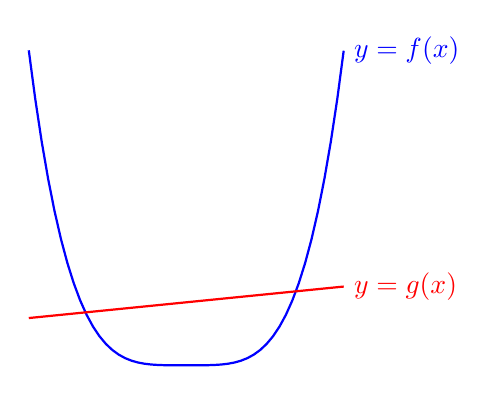
\begin{tikzpicture}
\YEaaxis{1}{5}{1}{5}
\YExcoord{4}{4}
\YEycoord{0.8}{A}
\draw[thick, blue] plot[domain=0:4, samples=50](\x,{pow({\x-2},4)/4})node[right]{$y=f(x)$};
\draw[thick, red] (0,.6)--(4,1) node[right]{$y=g(x)$};
\end{tikzpicture}
\end{center}
\begin{enumerate}[(a)]
\item Which function has a larger average on $[0,4]$:  $f(x)-A$ or  $g(x)-A$?
\item Which function has a larger average on $[0,4]$:  $|f(x)-A|$ or  $|g(x)-A|$?
\end{enumerate}
\end{Mquestion}
\begin{hint}
This is an application of the ideas in Question~\ref{prob_s2.2:var}.
\end{hint}
\begin{answer}
(a) neither--both are zero
\qquad
(b) $|f(x)-A|$ has the larger average on $[0,4]$
\end{answer}
\begin{solution}
\begin{enumerate}[(a)]
\item Neither: the average of both these functions is zero. We saw this with a particular function in Question~\ref{prob_s2.2:var} (b), but it's  actually true in general. It's a quick calculation to prove.

The average of $f(x)-A$ is:
\begin{align*}
\frac{1}{4-0}\int_0^4 \big(f(x)-A\big)\,\dee{x}&=\underbrace{\frac{1}{4}\int_0^4f(x)\,\dee{x}}_{A} - A=A-A=0
\end{align*}
Similarly, the average of $g(x)-A$ is:
\begin{align*}
\frac{1}{4-0}\int_0^4 \big(g(x)-A\big)\,\dee{x}&=\underbrace{\frac{1}{4}\int_0^4g(x)\,\dee{x}}_{A} - A=A-A=0
\end{align*}
\item The function $|f(x)-A|$ tells us how far $f(x)$ is from $A$, without worrying whether $f(x)$ is larger or smaller. Looking at our graph, for most values of $x$ in $[0,4]$, $f(x)$ is quite far away from $A$, so $|f(x)-A|$ is usually a large, positive quantity.

By contrast, $|g(x)-A|$ is a small positive quantity for most values of $x$. The function $g(x)$ is quite close to $A$ for all values of $x$ in $[0,4]$.

So, since $|g(x)-A|$ generally has much smaller values than $|f(x)-A|$, the average of $|f(x)-A|$ on $[0,4]$ will be larger than
the average of $|g(x)-A|$ on $[0,4]$.

As discussed in Question~\ref{prob_s2.2:var}(c), the average of $|f(x)-A|$ is a measure of how closely $f(x)$ resembles its average. We see from the graph that $f(x)$ doesn't resemble the constant function $y=A$ much at all, while $g(x)$ seems much more similar to the constant function $y=A$.

This kind of measure--how similar a function is to its average--is also the idea behind the root square mean.
\end{enumerate}
\end{solution}
%%%%%%%%%%%%%%%%%%%
\begin{question}
Suppose the root mean square of a function $f(x)$ on the interval $[a,b]$ is $R$. What is the volume of the solid formed by rotating the portion of $f(x)$ from $a$ to $b$ about the $x$-axis?
\begin{center}
\begin{tikzpicture}
\YEaaxis{2.5}{4}{2}{2}
\YExcoord{-1}{a}
\YEnxcoord{3}{b}
%\draw[blue, <->] (-1.5,.1)arc(20:340:2mm and 4mm);
%%%%%%%%%%%%%%%%%%%%%%%%%%%%%%%%%%%%%%%
\draw (-1,0) node[shape=ellipse, minimum width=0.5cm, minimum height = 2.08cm, draw]{};
\draw (0,.65) arc(90:-90:.125cm and .65cm);
\draw (3,1.21) arc(90:-90:.3cm and 1.21cm);
\draw[dashed] (0,.65) arc(90:270:.125cm and .65cm);
\draw[dashed] (3,1.21) arc(90:270:.3cm and 1.21cm);
%%%%%%%%%%%%%%%%%%%%%%%%%%%%%%%%%%%%%%%
\fill[fill opacity=.4, top color=black, bottom color=black, middle color=white] (-1,-1.04) arc(-90:90:0.26 cm and 1.04cm) plot[samples=100,domain=-1:0](\x,{(sqrt(abs(\x)))*cos(\x r)+.5})--(0,.65) arc (90:-90:.125cm and .65 cm)
--plot[domain=0:-1] (\x,{(-sqrt(abs(\x)))*cos(\x r)-.5});
\fill[fill opacity=.4, top color=black, bottom color=black, middle color=white] (0,-.65) arc(-90:90:0.125 cm and 0.65cm) plot[samples=100,domain=0:1.9](\x,{(sqrt(abs(\x)))*cos(\x r)+.5})
--plot[domain=1.9:0] (\x,{(-sqrt(abs(\x)))*cos(\x r)-.5});
\fill[fill opacity=.4, top color=black, bottom color=black, middle color=white]  plot[samples=100,domain=1.9:3](\x,{(sqrt(abs(\x)))*cos(\x r)+.5})arc(-90:90:0.3 cm and 1.21cm)
--plot[domain=3:1.9] (\x,{(-sqrt(abs(\x)))*cos(\x r)-.5});
\draw (-1,0) node[fill, fill opacity=0.3, shape=ellipse, minimum height=2.08cm, minimum width=0.52cm]{};
%%%%%%%%%%%%%%%%%%%%%%%%%%
\draw[very thick, blue] plot[samples=100,domain=-1.5:3.2](\x,{(sqrt(abs(\x)))*cos(\x r)+.5});
\draw plot[samples=100,domain=-1:3](\x,{-(sqrt(abs(\x)))*cos(\x r)-.5});
\draw[blue] (3.25,-1)node[below right]{$y=f(x)$};
\end{tikzpicture}
\end{center}
As in Example~\eref{CLP101}{eg:peakvsrms} of the CLP--II text, let the root mean square of $f(x)$ on $[a,b]$ be $\displaystyle\sqrt{\frac{1}{b-a}\int_a^b f^2(x)\,\dee{x}}$.
\end{question}
\begin{hint}
Slice the solid into circular disks of radius $|f(x)|$ and thickness $\dee{x}$.
\end{hint}
\begin{answer}
$(b-a)\pi R^2$
\end{answer}
\begin{solution}
When we rotate $f(x)$ about the $x$-axis, we form a solid whose radius at $x$ is $|f(x)|$. So, its circular cross-sections have area $\pi|f(x)|^2 = \pi f^2(x)$. If we slice this solid into circular disks of thickness $\dee{x}$, then the disks have volume $\pi f^2(x)\,\dee{x}$. Therefore, the volume of the entire solid is $\displaystyle\int_a^b \pi f^2(x)\,\dee{x}$. All we need to do now is get this into a form where we can replace the integral with the root mean square, $R$.
\begin{align*}
V&=\int_a^b \pi f^2(x)\,\dee{x} = \pi\frac{b-a}{b-a}\int_a^b f^2(x)\,\dee{x}\\
&=\pi(b-a)\left(\sqrt{\frac{1}{b-a}\int_a^b f^2(x)\,\dee{x}}\right)^2\\
&=\pi(b-a)R^2
\end{align*}
Remark: the volume of a cylinder with length $b-a$ and radius $r$ is $\pi(b-a)r^2$. So, the root mean square of $f(x)$ gave us the radius of a cylinder with the same volume as the solid formed by rotating $f(x)$. Recall the average of $f(x)$ gave us the height of a rectangle with the same area as $f(x)$. Compare this to the geometric interpretations of averages in Questions \ref{prob_s2.2:avgvalue} and \ref{prob_s2.2:avgarea}.
\end{solution}
%%%%%%%%%%%%%%%%%%%



%%%%%%%%%%%%%%%%%%%
\begin{question}\label{prob_s2.2:quadraticaverage}
Suppose $f(x)=ax^2+bx+c$, and the average value of $f(x)$ on the interval $[0,1]$ is the same as the average of $f(0)$ and $f(1)$. What is $a$?
\end{question}
\begin{hint}
The question tells you $\frac{1}{1-0}\int_0^1 f(x)\,\dee{x} = \frac{f(0)+f(1)}{2}$.
\end{hint}
\begin{answer}
0
\end{answer}
\begin{solution}
The question tells you $\frac{1}{1-0}\int_0^1 f(x)\,\dee{x} = \frac{f(0)+f(1)}{2}$. Note $f(0)=c$, and $f(1) = a+b+c$.
\begin{align*}
\frac{1}{1-0}\int_0^1 f(x)\,\dee{x} &= \frac{f(0)+f(1)}{2} = \frac{c+(a+b+c)}{2}\\
\int_0^1 \big(ax^2+bx+c \big)\,\dee{x}&=\frac{a+b+2c}{2}\\
\left[\frac{a}{3}x^3+\frac{b}{2}x^2+cx \right]_0^1&=\frac{a}{2}+\frac{b}{2}+c
\\\frac{a}{3}+\frac{b}{2}+c&=\frac{a}{2}+\frac{b}{2}+c\\
\frac{a}{3}&=a\\
a&=0
\end{align*}
That is, $f(x)$ is linear.
\end{solution}
%%%%%%%%%%%%%%%%%%%

\begin{question}
Suppose $f(x)=ax^2+bx+c$, and the average value of $f(x)$ on the interval $[s,t]$ is the same as the average of $f(s)$ and $f(t)$. Is it possible that $a \neq 0$?

That is--
does the result of Question~\ref{prob_s2.2:quadraticaverage} generalize?
\end{question}
\begin{hint}
Set up this question just like Question~\ref{prob_s2.2:quadraticaverage}, but with variables for your limits of integration.

Note $(s-t)^2=s^2-2st+t^2$.
\end{hint}
\begin{answer}
Yes, but if $a\neq0$, then $s=t$.
\end{answer}
\begin{solution}
The information given in the question is:
\begin{align*}
\frac{\big(as^2+bs+c\big)+\big(at^2+bt+c\big)}{2}&=\frac{1}{t-s}\int_s^t \big(ax^2+bx+c\big)\,\dee{x}\\
&=\frac{1}{t-s}\left[\frac{a}{3}x^3+\frac{b}{2}x^2+cx\right]_s^t
\\&=\frac{1}{t-s}\left[\frac{a}{3}(t^3-s^3)+\frac{b}{2}(t^2-s^2)+c(t-s)\right]\\
&=\frac{a}{3}(t^2+st+s^2)+\frac{b}{2}(t+s)+c\\
\frac{a}{2}(s^2+t^2) +\textcolor{red}{ \frac{b}{2}(s+t)}+\textcolor{blue}{c}&=\frac{a}{3}(t^2+st+s^2)+\textcolor{red}{\frac{b}{2}(t+s)}+\textcolor{blue}{c}\\
\frac{a}{2}(s^2+t^2)&=\frac{a}{3}(t^2+st+s^2)\\
a\left[\frac{s^2+t^2}{2} - \frac{t^2+st+s^2}{3}\right]&=0\\
a\left[\frac{s^2-2st+t^2}{6}\right]&=0
\\a(s-t)^2&=0\\
a&=0 \quad\text{OR}\quad s=t
\end{align*}
So, unless $s=t$ (and we're taking the very boring average of a single point!) then $a=0$. That is: $f(x)$ is linear whenever $s \neq t$.
\end{solution}


%%%%%%%%%%%%%%%%%%%
\begin{question}
Let $f(x)$ be a function defined for all numbers in the interval $[a,b]$, with average value $A$ over that interval. What is the average of $f(a+b-x)$ over the interval $[a,b]$?
\end{question}
\begin{hint}
What are the graphs of $f(x)$ and $f(a+b-x)$ like?
\end{hint}
\begin{answer}
$A$
\end{answer}
\begin{solution}
The function $g(x)=f(a+b-x)$, on the interval $[a,b]$, is a mirror of the function $f(x)$, with $g(a)=f(b)$ and $g(b)=f(a)$. So, $\int_a^b f(a+b-x)\,\dee{x} = \int_a^bf(x)\,\dee{x}$, and hence $\frac{1}{b-a}\int_a^b f(a+b-x)\,\dee{x} = \frac{1}{b-a}\int_a^bf(x)\,\dee{x}$, so the average value of $f(a+b-x)$ on $[a,b]$ is $A$.

Alternately, we can evaluate $\frac{1}{b-a}\int_a^b f(a+b-x)\,\dee{x}$ directly, using the substitution $u=a+b-x$, $\dee{x}=-\dee{x}$:
\begin{align*}
\frac{1}{b-a}\int_a^b f(a+b-x)\,\dee{x}&=\frac{-1}{b-a}\int_{u(a)}^{u(b)} f(u)\,\dee{u}\\
&=\frac{-1}{b-a}\int_{b}^{a} f(u)\,\dee{u}
\\&=\frac{1}{b-a}\int_{a}^{b} f(u)\,\dee{u}
\\&=A
\end{align*}
\end{solution}

%%%%%%%%%%%%%%%%%%%



\begin{question}
Suppose $f(t)$ is a continuous function, and
$A(x)$ is the average of $f(t)$ on the interval from 0 to $x$.
\begin{enumerate}[(a)]
\item What is the average of $f(t)$ on $[a,b]$, where $a<b$? Give your answer in terms of $A$.
\item What is $f(t)$? Again, give your answer in terms of $A$.
\end{enumerate}
\end{question}
\begin{hint}
For (b), express $A(x)$ as an integral, then differentiate.
\end{hint}
\begin{answer}
(a) $\displaystyle\frac{bA(b) - aA(a)}{b-a}$
\qquad
(b) $f(t)=A(t)+tA'(t) $
\end{answer}
\begin{solution}
\begin{enumerate}[(a)]
\item  The function $A(x)$ only gives us information about an integral when one limit of integration is zero. We can get around this by using properties of definite integrals from Section 1.2 to break our integral into two integrals, each of which has 0 as one limit of integration. So, we find the average of $f(t)$ on $[a,b]$ as follows:
\begin{align*}
\frac{1}{b-a}\int_a^b f(t)\,\dee{t}&=
\frac{1}{b-a}\left(\int_a^0 f(t)\,\dee{t} + \int_0^b f(t)\,\dee{t}\right)\\
&=\frac{1}{b-a}\left(-\int_0^a f(t)\,\dee{t} + \int_0^b f(t)\,\dee{t} \right)\\
&=\frac{1}{b-a}\left(-a\cdot\underbrace{\frac{1}{a}\int_0^a f(t)\,\dee{t}}_{A(a)} + b\cdot\underbrace{\frac{1}{b}\int_0^b f(t)\,\dee{t}}_{A(b)} \right)\\
&=\frac{1}{b-a}\left(-aA(a)+bA(b) \right) = \frac{bA(b) - aA(a)}{b-a}
\end{align*}
\item From the definition of $A(x)$, we know
\[A(x) = \frac{1}{x}\int_0^x f(t)\,\dee{t}\]
That is,
\[xA(x) =\int_0^x f(t)\,\dee{t}\]
To find $f(x)$, we differentiate both sides. For the left side, we use the product rule; for the right side, we use the Fundamental Theorem of Calculus part 1.
\[A(x)+xA'(x) = f(x)\]
So, $f(t)=A(t)+tA'(t)$.
\end{enumerate}
\end{solution}
%%%%%%%%%%%%%%%%%%%

\begin{Mquestion}
\begin{enumerate}[(a)]
\item Find a function $f(x)$ with average $0$ over $[-1,1]$ but $f(x) \neq 0$ for all $x$ in $[-1,1]$, or show that no such function exists.
\item Find a \emph{continuous} function $f(x)$ with average $0$ over $[-1,1]$ but $f(x) \neq 0$ for all $x$ in $[-1,1]$, or show that no such function exists.
\end{enumerate}
\end{Mquestion}
\begin{hint}
For (b), consider the cases that $f(x)$ is always bigger or always smaller than 0. Then, use the intermediate value theorem, Theorem~\eref{CLP100}{thm ivt} in the CLP--I text.
\end{hint}
\begin{answer}
\begin{enumerate}[(a)]
\item One of many possible answers: $f(x) = \begin{cases}
-1&\text{ if } x \leq 0\\
1&\text{ if } x > 0
\end{cases}$.
\item No such function exists.
\begin{description}
\item[Note 1:] Suppose $f(x)>0$ for all $x$ in $[-1,1]$. Then $\frac{1}{2}\int_{-1}^1f(x)\,\dee{x} > \frac{1}{2}\int_{-1}^10\,\dee{x} =0 $. That is, the average value of $f(x)$ on the interval $[-1,1]$ is not zero--it's something greater than zero.
\item[Note 2:] Suppose $f(x)<0$ for all $x$ in $[-1,1]$. Then $\frac{1}{2}\int_{-1}^1f(x)\,\dee{x} < \frac{1}{2}\int_{-1}^10\,\dee{x} =0 $. That is, the average value of $f(x)$ on the interval $[-1,1]$ is not zero--it's something less than zero.
\end{description}
So, if the average value of $f(x)$ is zero, then $f(x)\ge 0$ for some $x$ in $[-1,1]$, and $f(y) \le 0$ for some $y \in [-1,1]$. Since $f$ is a continuous function, and 0 is between $f(x)$ and $f(y)$, by the intermediate value theorem (Theorem~\eref{CLP100}{thm ivt} in the  in the CLP--I text) there is some value $c$ between $x$ and $y$ such that $f(c)=0$. Since $x$ and $y$ are both in $[-1,1]$, then $c$ is as well. Therefore, no function exists as described in the question.
\end{enumerate}
\end{answer}
\begin{solution}
\begin{enumerate}[(a)]
\item One of many possible answers: $f(x) = \begin{cases}
-1&\text{ if } x \leq 0\\
1&\text{ if } x > 0
\end{cases}$.
\item No such function exists.
\begin{description}
\item[Note 1:] Suppose $f(x)>0$ for all $x$ in $[-1,1]$. Then $\frac{1}{2}\int_{-1}^1f(x)\,\dee{x} > \frac{1}{2}\int_{-1}^10\,\dee{x} =0 $. That is, the average value of $f(x)$ on the interval $[-1,1]$ is not zero--it's something greater than zero.
\item[Note 2:] Suppose $f(x)<0$ for all $x$ in $[-1,1]$. Then $\frac{1}{2}\int_{-1}^1f(x)\,\dee{x} < \frac{1}{2}\int_{-1}^10\,\dee{x} =0 $. That is, the average value of $f(x)$ on the interval $[-1,1]$ is not zero--it's something less than zero.
\end{description}
So, if the average value of $f(x)$ is zero, then $f(x)\ge 0$ for some $x$ in $[-1,1]$, and $f(y) \le 0$ for some $y \in [-1,1]$. Since $f$ is a continuous function, and 0 is between $f(x)$ and $f(y)$, by the intermediate value theorem (Theorem~\eref{CLP100}{thm ivt} in the CLP--I text) there is some value $c$ between $x$ and $y$ such that $f(c)=0$. Since $x$ and $y$ are both in $[-1,1]$, then $c$ is as well. Therefore, no function exists as described in the question.
\end{enumerate}
\end{solution}
%%%%%%%%%%%%%%%%%%%
\begin{question}\label{prob_s2.2:limitavg}
Suppose $f(x)$ is a positive, continuous function with $\lim\limits_{x \to \infty} f(x)=0$, and let $A(x)$ be the average of $f(x)$ on $[0,x]$.

True or false: $\lim\limits_{x \to \infty} A(x) = 0$.
\end{question}
\begin{hint}
Try l'H\^{o}pital's rule.
\end{hint}
\begin{answer}
true
\end{answer}
\begin{solution}
This seems like it might be true: if $f$ is getting closer and closer to zero, as $x$ grows towards infinity, then over time the later values will become a larger and larger portion of the total interval we're looking at, and so the average should look more and more like $f(x)$ when $x$ is large--that is, like 0. That's some intuition to start us out, but it isn't a rigorous argument. To be sure we haven't overlooked something, let's use the definition of an average to express $A(x)$.
\begin{align*}
A(x)&=\frac{1}{x}\int_0^x f(t)\,\dee{t}\\
\lim_{x \to \infty}A(x)&=\lim_{x \to \infty}\frac{1}{x}\int_0^x f(t)\,\dee{t}
\intertext{If $\int_0^\infty f(t) \,\dee{t}$ converges, then this limit is 0, and the statement is true. So, suppose it does not converge. Since $f(x)$ is positive, that means $\lim\limits_{x \to \infty} \int_0^x f(t)\,\dee(t) = \infty$, so we can use l'H\^{o}pital's rule. To differentiate the numerator, we use the Fundamental Theorem of Calculus part 1.}
\lim_{x \to \infty}A(x)&=\lim_{x \to \infty}\frac{\int_0^x f(t)\,\dee{t}}{x} = \lim_{x \to \infty}\frac{f(t)}{1}=0
\end{align*}
So, the statement is true whether $\int_0^xf(t)\,\dee{t}$ converges or not.
\end{solution}
%%%%%%%%%%%%%%%%%%%


\begin{question}
Let $A(x)$ be the average of the function $f(t)=e^{-t^2}$ on the interval $[0,x]$. What is $\displaystyle\lim_{x \to \infty} A(x)$?
\end{question}
\begin{hint}
Use the result of Question~\ref{prob_s2.2:limitavg}.
\end{hint}
\begin{answer}
0
\end{answer}
\begin{solution}
Note $f(t)$ is a continuous function that takes only positive values, and $\lim\limits_{t \to \infty} f(t)=0$. By  the result of Question~\ref{prob_s2.2:limitavg}, $\displaystyle\lim_{x \to \infty} A(x)=0$.
\end{solution}
